\section{Connecting proposals across a cut}\label{sec:connections}

For distinct spins $x,y$, write $c_G(x,y)$ for the heat-bath jump
rate. The stationary flow across a set $S$ is
\[
 Q_G^{\rm edge}(S,S^{\rm c})
 =\sum_{x\in S,\,y\notin S}\pi_G(x)c_G(x,y).
\]
Detailed balance makes the edge weights symmetric. We will show that
this flow cannot be too small when both sides carry appreciable
Gibbs mass. The proof joins two proposals with a common smoothing
base, then uses coverage to place their endpoints across the cut and
the likelihood estimate to keep the connecting configurations away
from its boundary.

\begin{proposition}[Balanced-cut flow]\label{prop:cuts}
With probability tending to one in the target disorder,
\[
 Q_G^{\rm edge}(S,S^c)>B_{\min}:=\exp(-n^{1-b/20})
 \quad\text{for every }S\text{ such that }
 \min(\pi_G(S),\pi_G(S^c))\ge n^{-d}.
 \tag{11}\label{eq:11}
\]
\end{proposition}

\begin{proof}
We divide the argument into the geometry of a putative low-flow cut,
the construction of a proposal sequence, and the two estimates that
make this sequence impossible.

\paragraph{A low-flow cut has a small enlarged boundary.}
For a sufficiently large fixed $C$, Gaussian quadratic-form tails on
a $1/4$-net give $\|W(G)\|\le C$ except with probability
$O(e^{-cn})$. On this event, every one-spin energy difference is
$O(\sqrt n)$. The heat-bath rate across any one-spin edge is therefore
at least $\exp(-O_\beta(\sqrt n))$.
If a cut has flow at most $B_{\min}$, its two-sided vertex boundary
$\partial S$ consequently has Gibbs mass at most
$2B_{\min}\exp(O_\beta(\sqrt n))$.

Set $R_n=\lceil n^{1-b/4}\rceil$ and enlarge this boundary by
Hamming distance $R_n$. For two spins at that distance,
$\|W(G)\|\le C$ and their Euclidean distance bound the logarithmic
Gibbs weight ratio by $O_\beta(n^{1-b/8})$. A Hamming ball of radius
$R_n$ has logarithmic cardinality $O(n^{1-b/4}\log n)$.
The enlarged boundary therefore has target Gibbs mass at most
\[
 \exp(-\tfrac12n^{1-b/20}).
 \tag{12}\label{eq:12}
\]

Among cuts violating \eqref{eq:11}, select the first one in a fixed
ordering whenever such a cut exists and $\|W(G)\|\le C$.
Let $\mathcal D(G)$ be its enlarged boundary, and set
$\mathcal D(G)=\varnothing$ otherwise. This is a measurable
selection because the cube has finitely many subsets.
Let $\mathcal E$ be the event that a witness exists, the target
norm bound holds, and \eqref{eq:10} holds for the sampled base
$G^\circ$. The norm and coverage estimates reduce the proposition
to proving $\Pr(\mathcal E)=o(1)$.

\paragraph{A sequence with independent fine endpoints.}
The fine horizon $l=f$ and the coarse horizon $l=b$ serve different
purposes. On $\mathcal E$,
Proposition~\ref{prop:coverage} gives each side of the cut fine-proposal
probability at least $\exp(-n^{1-2d})$. Two conditionally independent
fine endpoints therefore cross the cut with probability at least
$\exp(-2n^{1-2d})$. We need an unconditional bound on failures of
the connecting sequence that is smaller than this endpoint probability.
The available fine-horizon exception bound
$\exp(-n^{1-10f})$ is not strong enough for this comparison; the
coarse bound $\exp(-n^{1-10b})$ is, since $10b<d/2<2d$.
We therefore use fine spins at the endpoints and coarse spins along
the grid. Their shared path prefixes and the magnetization martingale
will keep each fine endpoint close to its coarse output.

Given the target $G$ and base $G^\circ$, introduce independent
standard Gaussian vectors $G'_1,G'_2$, independent of both, and set
\[
 G(\theta)=\sqrt{1-\delta}\,G^\circ+
       \sqrt\delta(\cos\theta\,G'_1+\sin\theta\,G'_2),
 \qquad 0\le\theta\le\pi/2.
\]
Use a deterministic equally spaced grid including $0,\pi/2$, with
spacing $O(\exp(-n^{1/4}))$ and cardinality
$O(\exp(n^{1/4}))$. Rotate two independent collections of all
auxiliary Gaussian path inputs by the same cosine-sine rule.
At each grid point, run the proposal to the coarse horizon
\[
 V_b=h\lceil b\log n/h\rceil
\]
and draw its coarse spin. At each endpoint, also continue the path
to $V_f=h\lceil f\log n/h\rceil$ and draw a fine spin. Coarse
spin draws are not used in the continuation. All final spin draws
may use fresh independent randomness.

The two fine endpoint spins are independent conditional on
$(G,G^\circ)$ and have law $\nu(\cdot\mid G^\circ)$.
For each individual angle, averaging the disorder and auxiliary
inputs gives the appropriate proposal law. Its primitive auxiliary
collection is independent of all the target, base, and proposal
matrix drivers. The one-point estimates and their union bound require
no independence across grid points. The shared rotation will instead
supply the nearby inputs needed for continuity along the grid.

We prove that, outside an event of probability at most
$\exp(-n^{1-d/2})$, the following two properties hold:
\begin{enumerate}
\item Every coarse spin avoids $\mathcal D(G)$.
\item The sequence formed by the first fine spin, all coarse spins in
grid order, and the last fine spin has consecutive Hamming distances
at most $R_n$.
\end{enumerate}
The probability here is unconditional. Figure~\ref{fig:connection}
shows the deterministic obstruction these properties create when the
fine endpoints lie on opposite sides of a cut.
\begin{figure}[!htbp]
\centering
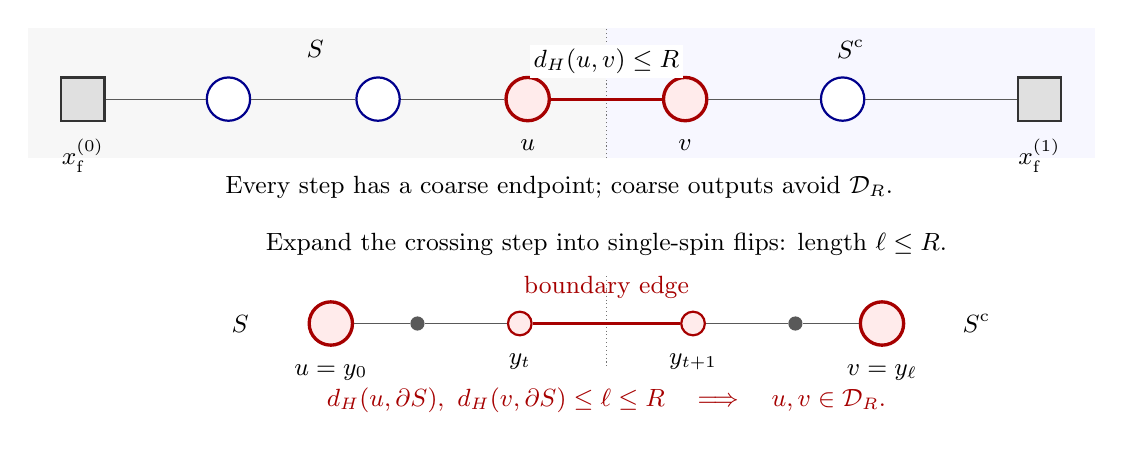
\begin{tikzpicture}[
  x=1cm,y=1cm,font=\small,
  coarse/.style={circle,draw=blue!55!black,fill=white,
    line width=.8pt,minimum size=5.5mm,inner sep=0pt},
  fine/.style={rectangle,draw=black!80,fill=black!12,
    line width=.8pt,minimum size=5.5mm,inner sep=0pt},
  forced/.style={coarse,draw=red!65!black,fill=red!8,line width=1.2pt},
  flip/.style={circle,fill=black!65,minimum size=1.8mm,inner sep=0pt},
  boundary/.style={circle,draw=red!65!black,fill=red!8,
    line width=.8pt,minimum size=3mm,inner sep=0pt}
]
  \fill[black!3] (-.05,-.75) rectangle (7.3,.9);
  \fill[blue!3] (7.3,-.75) rectangle (13.5,.9);
  \draw[densely dotted,black!55] (7.3,-.75) -- (7.3,.9);
  \node at (3.6,.63) {$S$};
  \node at (10.4,.63) {$S^{\mathrm c}$};

  \node[fine] (leftfine) at (.65,0) {};
  \node[coarse] (coarsezero) at (2.5,0) {};
  \node[coarse] (coarseone) at (4.4,0) {};
  \node[forced] (crossleft) at (6.3,0) {};
  \node[forced] (crossright) at (8.3,0) {};
  \node[coarse] (coarselast) at (10.3,0) {};
  \node[fine] (rightfine) at (12.8,0) {};
  \draw[black!65] (leftfine) -- (coarsezero)
    (coarsezero) -- (coarseone) (coarseone) -- (crossleft)
    (crossright) -- (coarselast) (coarselast) -- (rightfine);
  \draw[red!65!black,line width=1.1pt] (crossleft) -- (crossright);
  \node[below=1mm] at (leftfine.south) {$x_{\rm f}^{(0)}$};
  \node[below=1mm] at (rightfine.south) {$x_{\rm f}^{(1)}$};
  \node[below=1mm] at (crossleft.south) {$u$};
  \node[below=1mm] at (crossright.south) {$v$};
  \node[fill=white,inner sep=1.5pt] at (7.3,.48)
    {$d_H(u,v)\le R$};
  \node at (6.7,-1.12)
    {Every step has a coarse endpoint; coarse outputs avoid $\mathcal D_R$.};

  \node at (7.3,-1.85)
    {Expand the crossing step into single-spin flips: length $\ell\le R$.};
  \draw[densely dotted,black!55] (7.3,-2.25) -- (7.3,-3.4);
  \node[forced] (pathleft) at (3.8,-2.85) {};
  \node[flip] (pathone) at (4.9,-2.85) {};
  \node[boundary] (boundaryleft) at (6.2,-2.85) {};
  \node[boundary] (boundaryright) at (8.4,-2.85) {};
  \node[flip] (pathlast) at (9.7,-2.85) {};
  \node[forced] (pathright) at (10.8,-2.85) {};
  \draw[black!65] (pathleft) -- (pathone) (pathone) -- (boundaryleft)
    (boundaryright) -- (pathlast) (pathlast) -- (pathright);
  \draw[red!65!black,line width=1.1pt] (boundaryleft) -- (boundaryright);
  \node[above=2mm,red!65!black] at (7.3,-2.85) {boundary edge};
  \node[below=1mm] at (pathleft.south) {$u=y_0$};
  \node[below=1mm] at (boundaryleft.south) {$y_t$};
  \node[below=1mm] at (boundaryright.south) {$y_{t+1}$};
  \node[below=1mm] at (pathright.south) {$v=y_\ell$};
  \node at (2.65,-2.85) {$S$};
  \node at (12,-2.85) {$S^{\mathrm c}$};
  \node[red!65!black] at (7.3,-3.83)
    {$d_H(u,\partial S),\ d_H(v,\partial S)\le\ell\le R
      \quad\Longrightarrow\quad u,v\in\mathcal D_R$.};
\end{tikzpicture}
\caption{The boundary obstruction for the finite sequence of proposals.
In the upper chain, squares are fine endpoints and circles are coarse outputs; consecutive
configurations have Hamming distance at most $R$. When the fine endpoints lie on opposite sides, some consecutive pair
$u,v$ crosses the cut and contains a coarse output. A shortest path of
one-spin flips between that pair meets the two-sided boundary $\partial S$.
Its length is at most $R$, so both $u,v$ lie in
$\mathcal D_R=\{x:d_H(x,\partial S)\le R\}$, contradicting avoidance by
the coarse outputs. All geometry is schematic: grid outputs are
correlated, and lines do not represent continuous spin trajectories.}
\label{fig:connection}
\end{figure}


\paragraph{Avoiding a boundary selected from the target.}
At a fixed grid point, the driver difference $G-G(\theta)$ has
coordinate variance $2\delta$. Gaussian tails and a union bound over
spins show that the supremum of absolute energy differences is
$O(n\sqrt\delta)$, except with probability $O(e^{-cn})$.
On its complement, Gibbs weight ratios between the two disorders
are at most $\exp(O_\beta(n\sqrt\delta))$.

Apply the likelihood estimate \eqref{eq:6} with $l=b$. Its good
event depends only on this proposal run. If
$q_{\rm good}(dx\mid g)$ is the corresponding output
subprobability kernel, disintegration against the Gaussian disorder
marginal gives
\[
 q_{\rm good}(dx\mid g)
 \le\exp(n^{1-b/2})\pi_g(dx)
 \quad\text{for almost every }g.
\]
The primitive auxiliary inputs and final draw for this run are
independent of all matrix drivers. Thus, after fixing
$G(\theta)=g$ and adjoining $(G,G^\circ)$, this remains its
conditional good-output kernel. In particular, the inequality applies
to the random set $\mathcal D(G)$ once those matrices have been
fixed. The separate energy-change event is used to compare Gibbs
weights; it is not built into the proposal good event.

By \eqref{eq:12}, the resulting boundary probability on the
energy-change event's complement is at most
\[
 \exp\bigl(n^{1-b/2}+O_\beta(n\sqrt\delta)
                   -\tfrac12n^{1-b/20}\bigr).
\]
Add the proposal exceptional probability
$\exp(-n^{1-10b})$ and the energy-change exception. Since
$\sqrt\delta=n^{-f/8}$, this proves the required one-point
avoidance bound. Correlations with auxiliary inputs at other grid
points do not change this calculation.

\paragraph{Continuity of the coarse magnetizations.}
We next control the increments along the grid. At any grid point,
Proposition~\ref{prop:proposal} puts the Gram matrix of the coarse
$T_k$ within $n^{-b}$ of the identity except with probability
$\exp(-n^{1-10b})$. On this event all $|T_k|_n\le2$, and each
Gram--Schmidt residual has norm at least $1/2$. No fallback direction
is used. The reciprocals $1/s_k$ are bounded by a fixed power of $n$
on the deterministic coarse horizon, by \eqref{eq:1}.

For neighboring grid points satisfying these Gram conditions, we claim
\[
 |M_\theta(V_b)-M_{\theta'}(V_b)|_n
 \le(n^{C_1})^{K_b+1}|\theta-\theta'|,
 \qquad K_b=V_b/h,
 \tag{13}\label{eq:13}
\]
provided the primitive inputs have polynomially bounded norms.
The constant $C_1$ is independent of the grid and of $n$.

Here are the precise input bounds and the interval induction proving
this assertion. Bound the operator norms of
$W(G^\circ),W(G'_1),W(G'_2)$ and the normalized norms of all
completion vectors $z_k$ in the two input collections. For their
Brownian and bridge inputs, bound the supremum norms of cumulative
integrals against the deterministic coefficients $\rho$ and
$\sqrt{1-\rho^2}$. On a filled interval include only the centered
bridge in this primitive bound; its endpoint is handled separately.
All these norms are at most $n^3$ outside an event of probability
$O(e^{-cn})$. Gaussian tails give the matrix and vector estimates.
For the path integrals, write a bridge as Brownian motion minus
its linearly interpolated endpoint and use the Gaussian martingale
maximal bound for a bounded deterministic integrand. Rotation makes
the differences of the primitive inputs at two angles at most a
polynomial factor times $|\theta-\theta'|$.

At a Gram--Schmidt step, the difference of the two projection
operators is bounded by twice the sum of preceding direction
differences in $|\cdot|_n$. Normalizing residuals of norm at least
$1/2$ costs only a fixed factor. Using $1/s_k$, the new direction
difference is therefore controlled by earlier magnetization and
direction differences at polynomial cost. The same is true of the
new $g_k$, by its matrix-query and completion formula. The cumulative
driving signals from \eqref{eq:4} differ by the primitive integral
differences plus the endpoint difference multiplied by a deterministic
factor at most $\sqrt h$. Finally, the scalar integral equation
and its spatially Lipschitz drift control the differences in $Y$ and
$M$ over this interval at constant cost, by Gronwall's inequality.
Starting with the entirely auxiliary first interval and taking
successive maxima of these differences proves \eqref{eq:13} after
increasing $C_1$ if necessary.

Only the Gram conditions at the two endpoints of each grid step
were used. Since $K_b=O(n^{1/16}\log n)$ and the mesh spacing is
exponentially smaller, \eqref{eq:13} makes all consecutive coarse
magnetization differences negligible.

\paragraph{From magnetizations to spins.}
For either a coarse spin or a fine endpoint spin compared with its
own coarse magnetization, the normalized squared distance has mean
\[
 1-\mathbb E m_{V_b}^2=p(V_b)\le C_\beta n^{-b/2}.
\]
For a fine spin this follows from the martingale conditional mean
through the continuation. Under the unconditioned single-run law,
each squared distance is an average of bounded independent coordinate
variables. It is consequently at most $n^{-b/3}$ except with
probability $O(\exp(-n^{1-b}))$. The triangle inequality in
$|\cdot|_n$, together with the negligible magnetization increments,
then gives Hamming step sizes at most $R_n$ for large $n$.

We may now union bound all one-point and consecutive-point exceptions
for the two desired properties, including the primitive-input event.
The grid costs only $\exp(O(n^{1/4}))$, and $10b<d/2$.
The boundary exponent $1-b/20$ also exceeds $1-d/2$.
Thus the total failure probability is at most
$\exp(-n^{1-d/2})$ for sufficiently large $n$.

\paragraph{The crossing contradiction.}
On $\mathcal E$, Proposition~\ref{prop:coverage} gives each side of the
chosen cut fine-endpoint probability at least
$\exp(-n^{1-2d})$. Conditional independence therefore puts the
fine endpoints on opposite sides with probability at least
$\exp(-2n^{1-2d})$. But if both sequence properties hold, this
cannot happen. Some consecutive pair would cross the cut, and each
pair contains a coarse spin. A shortest one-spin path between that
pair meets $\partial S$ and has length at most $R_n$, placing
that coarse spin in $\mathcal D(G)$.

Consequently
\[
 \Pr(\mathcal E)\exp(-2n^{1-2d})
 \le\exp(-n^{1-d/2}).
\]
Since $d/2<2d$, this implies $\Pr(\mathcal E)=o(1)$ and proves
\eqref{eq:11}. The auxiliary diagonal and smoothing base are used
only in this proof; the resulting flow bound concerns the original
heat bath.
\end{proof}
